\documentclass[12pt,a4paper,twoside]{article}

\usepackage{amsmath,amssymb,amsthm}			% math packages
\usepackage{fontspec}						% fonts
\usepackage{bold-extra}
\usepackage[no-math]{luatexja-fontspec}
\usepackage{newpxtext,newpxmath}
\usepackage{mathtools}
\usepackage[hidelinks,colorlinks=false,bookmarks=true]{hyperref}
\usepackage{emoji}			% funny emoji	
\usepackage{geometry}
\usepackage{calc}
\usepackage{tikz}
\usepackage{ctable}   		% tabular
\usepackage{tabularx} 
\usepackage{wrapfig}  		% floating figure
\usepackage{karnaugh-map} 	% k-map
\usepackage{multicol}		% multicol for saving spaces
\usepackage{enumerate}		% better enumerate
\usepackage{listings}		% code blocks
\usepackage{array}
\usepackage{titling}
\usepackage{fancyhdr}
\usepackage{blindtext}
\usepackage{algpseudocodex}
\usepackage{graphicx}

\setmainjfont[BoldFont=Noto Sans CJK TC Bold]{Noto Sans CJK TC}
\setsansjfont[BoldFont=Noto Sans CJK TC Bold]{Noto Sans CJK TC}
\setemojifont{Twemoji Mozilla}


\geometry{
	includehead,includefoot,
	top=0cm,
	bottom=0.5cm,
	left=1cm,
	right=1cm
}
\pagestyle{fancy}
\fancyhead[RO,LE]{\thetitle}
\fancyhead[RE,LO]{\theauthor}

\setlength{\parindent}{0em}
\renewcommand{\baselinestretch}{1.2}
 
% tikz
\usetikzlibrary{automata,positioning,arrows}
\usetikzlibrary{graphs,graphdrawing,graphdrawing.trees}

% theorems
\theoremstyle{definition}
\newtheorem{theorem}{Theorem}[section]
\newtheorem{definition}{Definition}[section]
\newtheorem{property}{Property}[section]
\newtheorem{lemma}{Lemma}[section]
\newtheorem{claim}{Claim}[section]
\newtheorem*{remark}{Remark}
\theoremstyle{remark}
\newtheorem*{example}{Example}

% math conventional macro
\newcommand{\ve}{\varepsilon}
\newcommand{\overbar}[1]{\mkern1.5mu\overline{\mkern-1.5mu#1\mkern-1.5mu}\mkern1.5mu}
\renewcommand{\qedsymbol}{\(\blacksquare\)}

% binary conventional macro
\newcommand{\bin}{\textsubscript{2}\ }
\newcommand{\dec}{\textsubscript{10}\ }

\setlength{\droptitle}{-7em}
\posttitle{\par\end{center}                 \vspace{-1em}}
\postauthor{\end{tabular}\par\end{center}   \vspace{-1.5em}}
\postdate{\par\end{center}                  \vspace{-3em}}

\title{Data Structure and Algorithm \textbf{Final Note}}
\author{B12902057 王淇}
\date{}

\tikzset{B/.style={text=white,draw=black,fill=black,thick,circle,minimum size=2em}}
\tikzset{R/.style={text=white,draw=red!70!black,fill=red!70!black,thick,draw,circle,minimum size=2em}}
\tikzset{RB/.style={text=white,draw=brown,fill=brown,thick,draw,circle,minimum size=2em}}
\tikzset{NIL/.style={text=white,draw=black,fill=black,rectangle,font={\scriptsize NIL}}}
\tikzset{no border/.style={minimum size=1em,draw=none}}
\tikzgraphsset{RBtree/.style={binary tree layout, grow=down, fresh nodes, level distance=2em, 
                    level 1/.style={sibling distance=12em},
                    level 2/.style={sibling distance=8em},
                    level 3/.style={sibling distance=2em},
                    level 4/.style={sibling distance=0em}}}
\tikzgraphsset{RBtree shallow/.style={binary tree layout, grow=down, fresh nodes, level distance=2em, 
                    level 1/.style={sibling distance=10em},
                    level 2/.style={sibling distance=5em},
                    level 3/.style={sibling distance=2em},
                    level 4/.style={sibling distance=0em}}}


\begin{document}
	\section{RB Tree}
    \begin{multicols}{2}
        \subsection{Black Height}
        \begin{tikzpicture}[>=latex,baseline={([yshift=-.5ex]current bounding box.center)}]
            \graph [RBtree shallow]
            {
                2[B] -> {1[B] -> {1[R] -> {A/[NIL], A/[NIL]}, A/[NIL]}, 2[R] -> {1[B] -> {A/[NIL], A/[NIL]}, 1[B] -> {A/[NIL], A/[NIL]}}}
            };
        \end{tikzpicture}

        \subsection{Rotation}
        \begin{tikzpicture}[>=latex,every node/.style={draw, circle, minimum size=2em}, baseline={([yshift=-.5ex]current bounding box.center)}]
            \graph [RBtree shallow]
            {
                x -> {y -> {a/$\alpha$[draw=none], b/$\beta$[draw=none]}, c/$\gamma$[draw=none]} 
            };
        \end{tikzpicture}
        $\xrightleftharpoons[\text{Left rotate}]{\text{Right rotate}}$
        \begin{tikzpicture}[>=latex,every node/.style={draw, circle, minimum size=2em}, baseline={([yshift=-.5ex]current bounding box.center)}]
            \graph [RBtree shallow]
            {
                x -> {a/$\alpha$[draw=none], {y -> {b/$\beta$[draw=none], c/$\gamma$[draw=none]}}}
            };
        \end{tikzpicture}
    \end{multicols}

    \subsection{Insert Fixup}
    Loop invariant: Always red violation.

    
    \begin{multicols}{2}
        Case 1: \textbf Uncle is red (My \textbf Parent is left child)

        \vspace{1em}
        \begin{tikzpicture}[>=latex,every node/.style={draw, circle, minimum size=2em}, baseline={([yshift=-.5ex]current bounding box.center)}]
            \graph [RBtree shallow]
            {
                G[B] -> {P[R] -> {x[R, double], x'[R, double ]}, {U[R]}}
            };
        \end{tikzpicture}
        $\xrightarrow{\text{Recolor}}$
        \begin{tikzpicture}[>=latex,every node/.style={draw, circle, minimum size=2em}, baseline={([yshift=-.5ex]current bounding box.center)}]
            \graph [RBtree shallow]
            {
                G[R,double] -> {P[B] -> {x[R], x[R]}, {U[B]}}
            };
        \end{tikzpicture}
        \vspace{1.5em}

        Case 4: \textbf Uncle is red (My \textbf Parent is right child)
        
        \vspace{1em}
        \begin{tikzpicture}[>=latex,every node/.style={draw, circle, minimum size=2em}, baseline={([yshift=-.5ex]current bounding box.center)}]
            \graph [RBtree shallow]
            {
                G[B] -> {U[R], P[R] -> {x[R, double], x'[R, double]}}
            };
        \end{tikzpicture}
        $\xrightarrow{\text{Recolor}}$
        \begin{tikzpicture}[>=latex,every node/.style={draw, circle, minimum size=2em}, baseline={([yshift=-.5ex]current bounding box.center)}]
            \graph [RBtree shallow]
            {
                G[R,double] -> {U[B], P[B] -> {x[R], x[R]}}
            };
        \end{tikzpicture}
        \vspace{1.5em}
    \end{multicols}



    \begin{multicols}{2}
        Case 2: \textbf Uncle is black, I am his near nephew
    
        \vspace{1em}
        \begin{tikzpicture}[>=latex,every node/.style={draw, circle, minimum size=2em}, baseline={([yshift=-.5ex]current bounding box.center)}]
            \graph [RBtree shallow]
            {
                G[B] -> {P[R] -> {, x[R, double]}, {U[B]}}
            };
        \end{tikzpicture}
        $\xrightarrow{\text{Left Rotate}}$
        \begin{tikzpicture}[>=latex,every node/.style={draw, circle, minimum size=2em}, baseline={([yshift=-.5ex]current bounding box.center)}]
            \graph [RBtree shallow]
            {
                G[B] -> {x[R] -> {P[R, double], }, {U[B]}}
            };
        \end{tikzpicture}
        \vspace{1.5em}

        Case 5: \textbf Uncle is black, I am his near nephew
    
        \vspace{1em}
        \begin{tikzpicture}[>=latex,every node/.style={draw, circle, minimum size=2em}, baseline={([yshift=-.5ex]current bounding box.center)}]
            \graph [RBtree shallow]
            {
                G[B] -> {U[B], P[R] -> {x[R, double], }}
            };
        \end{tikzpicture}
        $\xrightarrow{\text{Right Rotate}}$
        \begin{tikzpicture}[>=latex,every node/.style={draw, circle, minimum size=2em}, baseline={([yshift=-.5ex]current bounding box.center)}]
            \graph [RBtree shallow]
            {
                G[B] -> {U[B], x[R] -> {, P[R, double]}}
            };
        \end{tikzpicture}
        \vspace{1.5em}
    \end{multicols}

    Case 3: \textbf Uncle is black, I am his distant nephew (my \textbf Parent is left child)
    \begin{flushright}
        Case 6: \textbf Uncle is black, I am right child (my \textbf Parent is right child)
    \end{flushright}

    \vspace{1em}
    \begin{tikzpicture}[>=latex,every node/.style={draw, circle, minimum size=2em}, baseline={([yshift=-.5ex]current bounding box.center)}]
        \graph [RBtree shallow]
        {
            G[B] -> {P[R] -> {x[R, double], }, {U[B]}}
        };
    \end{tikzpicture}
    $\xrightarrow{\text{Right Rotate}}$
    \begin{tikzpicture}[>=latex,every node/.style={draw, circle, minimum size=2em}, baseline={([yshift=-.5ex]current bounding box.center)}]
        \graph [RBtree shallow]
        {
            P[R] -> {x[R], G[B] -> {, U[B]}}
        };
    \end{tikzpicture}
    $\xrightarrow{\text{Recolor}}$
    \begin{tikzpicture}[>=latex,every node/.style={draw, circle, minimum size=2em}, baseline={([yshift=-.5ex]current bounding box.center)}]
        \graph [RBtree shallow]
        {
            P[B, double] -> {x[R], G[R] -> {, U[B]}}
        };
    \end{tikzpicture}
    \begin{flushright}
        \begin{tikzpicture}[>=latex,every node/.style={draw, circle, minimum size=2em}, baseline={([yshift=-.5ex]current bounding box.center)}]
            \graph [RBtree shallow]
            {
                G[B] -> {U[B], P[R] -> {, x[R, double]}}
            };
        \end{tikzpicture}
        $\xrightarrow{\text{Left Rotate}}$
        \begin{tikzpicture}[>=latex,every node/.style={draw, circle, minimum size=2em}, baseline={([yshift=-.5ex]current bounding box.center)}]
            \graph [RBtree shallow]
            {
                P[R] -> {G[B] -> {U[B], }, x[R]}
            };
        \end{tikzpicture}
        $\xrightarrow{\text{Recolor}}$
        \begin{tikzpicture}[>=latex,every node/.style={draw, circle, minimum size=2em}, baseline={([yshift=-.5ex]current bounding box.center)}]
            \graph [RBtree shallow]
            {
                P[B, double] -> {G[R] -> {U[B], }, x[R]}
            };
        \end{tikzpicture}
    \end{flushright}
    \vspace{1.5em}
    
    % Case 4: \textbf Uncle is red (my \textbf Parent is right child)
    % Case 5: \textbf Uncle is black, I am left child (my \textbf Parent is right child)
    % Case 6: \textbf Uncle is black, I am right child (my \textbf Parent is right child)

    \subsection{Delete}
    If target node has only one child, then move it up and call fixup. Otherwise, let current be $z$, next node be $y$, $y$ has only a child $x$. We move $y$'s key to $z$, and remove $y$ (child moves up). Call fixup on $y$.

    \subsection{Delete Fixup}
    Loop invariant: Subtree of current node always missing one black height.

    Case 0: I am red or root --- color myself to black, and terminate (fixup only need for black)
    \vspace{1em}

    Case 1: My \textbf Sibling is red 
    
    \vspace{1em}
    \begin{tikzpicture}[>=latex,baseline={([yshift=-.5ex]current bounding box.center)}]
        \graph [RBtree shallow]
        {
            P[B] -> {x[B,double] -> {"$-1$", "$-1$"}, S[R] -> {N[B], }}
        };
    \end{tikzpicture}
    $\xrightarrow{\text{Left Rotate}}$
    \begin{tikzpicture}[>=latex,baseline={([yshift=-.5ex]current bounding box.center)}]
        \graph [RBtree]
        {
            S[R] -> {P[B] -> {x[B] -> {"$-1$", "$-1$"}, N[B]}, "$-1$"}
        };
    \end{tikzpicture}
    $\xrightarrow{\text{Recolor}}$
    \begin{tikzpicture}[>=latex,baseline={([yshift=-.5ex]current bounding box.center)}]
        \graph [RBtree ]
        {
            S[B] -> {P[R] -> {x[B,double] -> {"$-1$", "$-1$"}, N[B]}, }
        };
    \end{tikzpicture}
    \vspace{1.5em}

    Case 2: My \textbf Sibling is black, and both its children are black

    \vspace{1em}
    \begin{tikzpicture}[>=latex,baseline={([yshift=-.5ex]current bounding box.center)}]
        \graph [RBtree shallow]
        {
            P[RB] -> {x[B,double], S[B] -> {N[B], D[B]}}
        };
    \end{tikzpicture}
    $\xrightarrow{\text{Recolor}}$
    \begin{tikzpicture}[>=latex,baseline={([yshift=-.5ex]current bounding box.center)}]
        \graph [RBtree shallow]
        {
            P[RB,double] -> {x[B], S[R] -> {N[B], D[B]}}
        };
    \end{tikzpicture}
    \vspace{1.5em}

    Case 3: My \textbf Sibling is black, and the \textbf Distant child is black

    \vspace{1em}
    \begin{tikzpicture}[>=latex,baseline={([yshift=-.5ex]current bounding box.center)}]
        \graph [RBtree shallow]
        {
            P[RB] -> {x[B,double] -> {"$-1$", "$-1$"}, S[B] -> {N[R], D[B]}}
        };
    \end{tikzpicture}
    $\xrightarrow{\text{Right Rotate}}$
    \begin{tikzpicture}[>=latex,baseline={([yshift=-.5ex]current bounding box.center)}]
        \graph [RBtree shallow]
        {
            P[RB] -> {x[B,double] -> {"$-1$", "$-1$"}, N[R] -> {"$-1$", S[B] -> {, D[B]}}}
        };
    \end{tikzpicture}
    $\xrightarrow{\text{Recolor}}$
    \begin{tikzpicture}[>=latex,baseline={([yshift=-.5ex]current bounding box.center)}]
        \graph [RBtree shallow]
        {
            P[RB] -> {x[B,double] -> {"$-1$", "$-1$"}, N[B] -> {, S[R] -> {, D[B]}}}
        };
    \end{tikzpicture}
    \vspace{1.5em}

    Case 4: My \textbf Sibling is black, and the \textbf Distant child is red

    \vspace{1em}
    \begin{tikzpicture}[>=latex,baseline={([yshift=-.5ex]current bounding box.center)}]
        \graph [RBtree shallow]
        {
            P[RB] -> {x[B,double] -> {"$-1$", "$-1$"}, S[B] -> {N[RB], D[R]}}
        };
    \end{tikzpicture}
    $\xrightarrow{\text{Left Rotate}}$
    \begin{tikzpicture}[>=latex,baseline={([yshift=-.5ex]current bounding box.center)}]
        \graph [RBtree shallow]
        {
            S[B] -> {P[RB] -> {x[B], N[RB]}, D[R] -> {"$-P$", "$-P$"}}
        };
    \end{tikzpicture}
    $\xrightarrow{\text{Recolor}}$
    \begin{tikzpicture}[>=latex,baseline={([yshift=-.5ex]current bounding box.center)}]
        \graph [RBtree shallow]
        {
            S[RB] -> {P[B] -> {x[B], N[RB]}, D[B]}
        };
    \end{tikzpicture}
    \clearpage
    \subsection{Pseudo Codes}
    \begin{multicols}{2}
		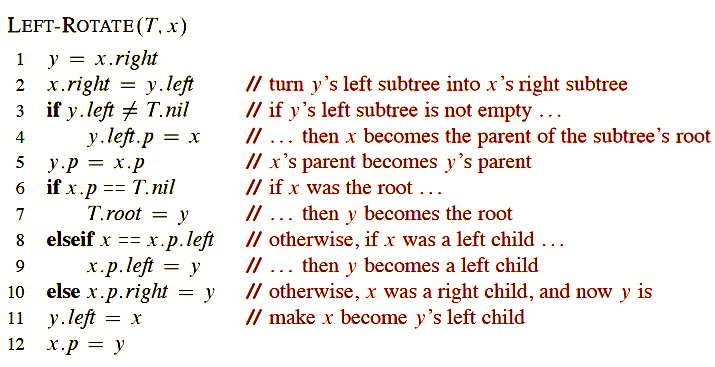
\includegraphics[width=.5\textwidth]{high-rb-lrot}
		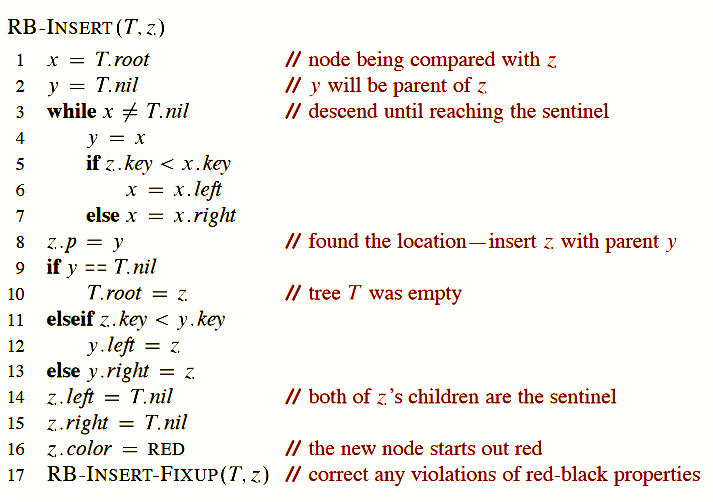
\includegraphics[width=.5\textwidth]{high-rb-insert}
		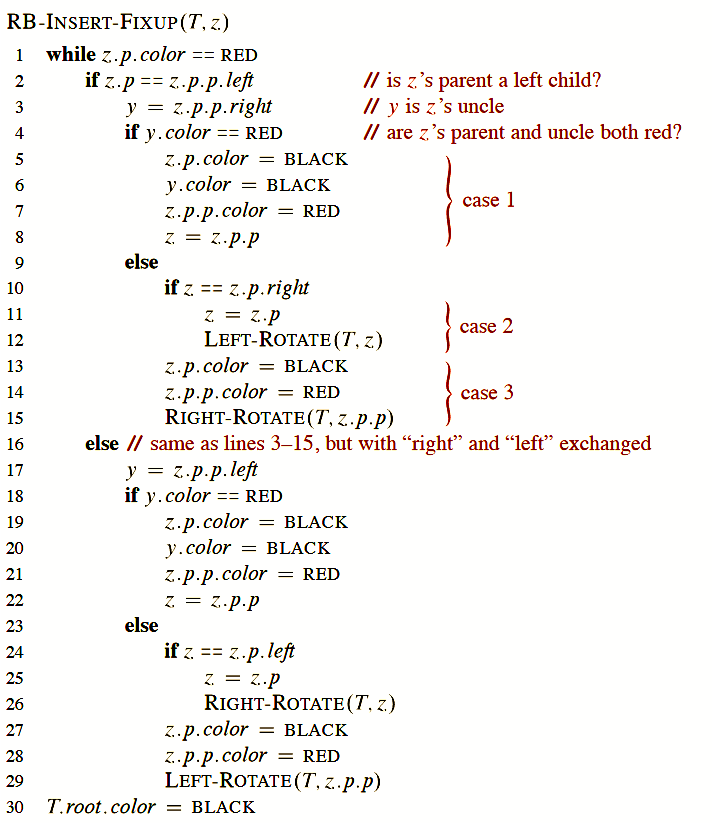
\includegraphics[width=.5\textwidth]{high-rb-insert-fix}
		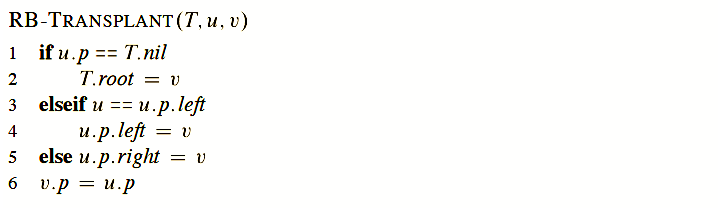
\includegraphics[width=.5\textwidth]{high-rb-transplant}
		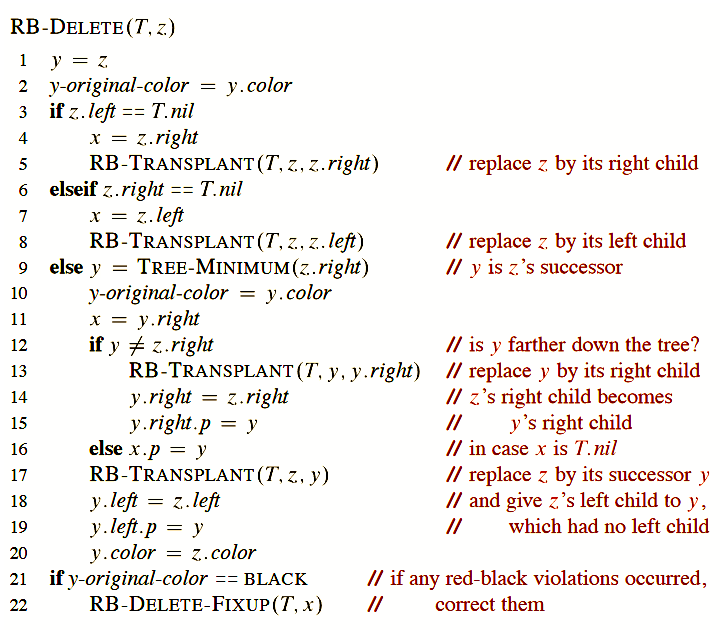
\includegraphics[width=.5\textwidth]{high-rb-delete}
		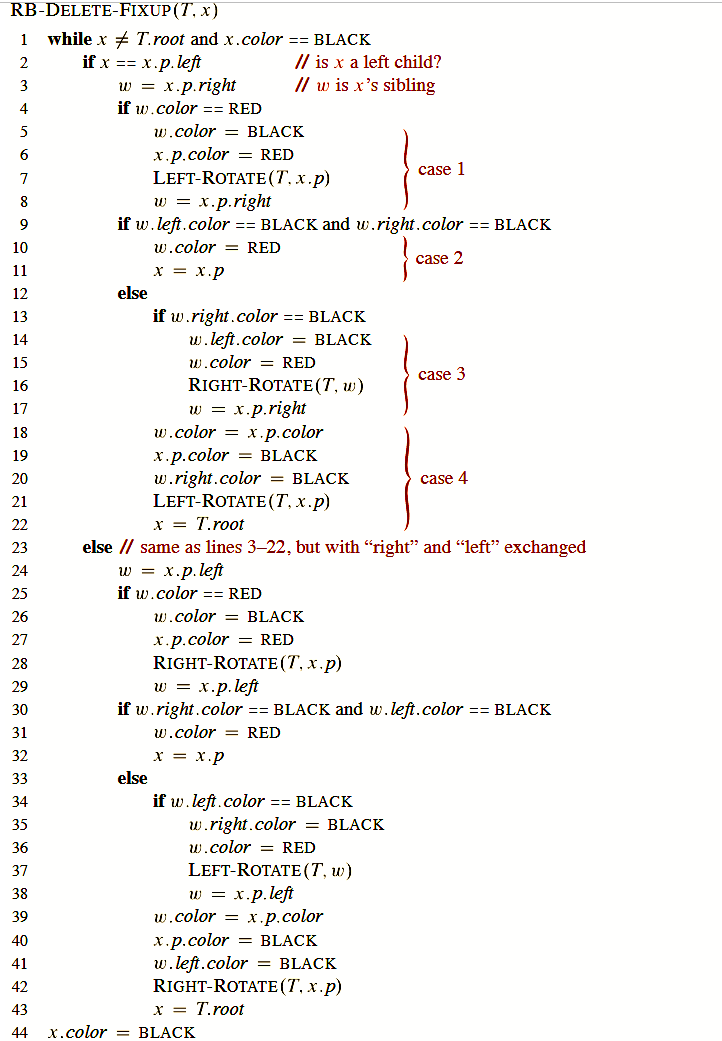
\includegraphics[width=.5\textwidth]{high-rb-delete-fixup}
    \end{multicols}
    \clearpage

	\section{B Tree}
    \subsection{Pseudo Codes}
    \begin{multicols}{2}
		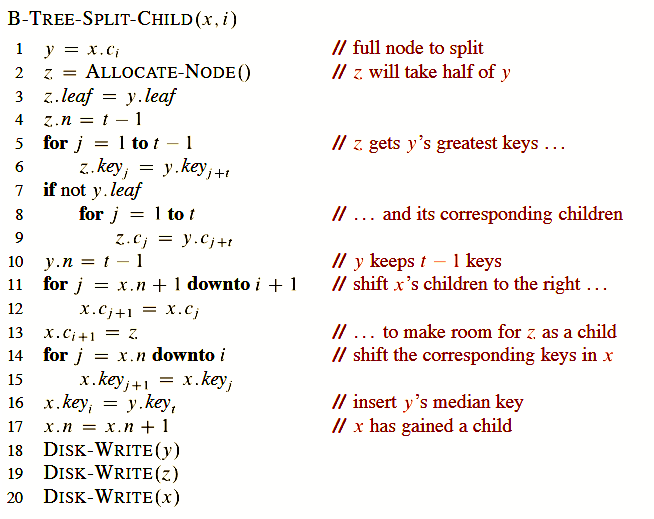
\includegraphics[width=.5\textwidth]{high-b-split-child}
		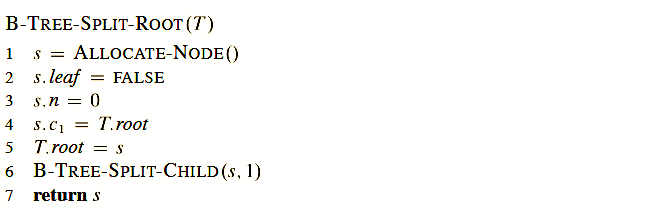
\includegraphics[width=.5\textwidth]{high-b-split-root}
		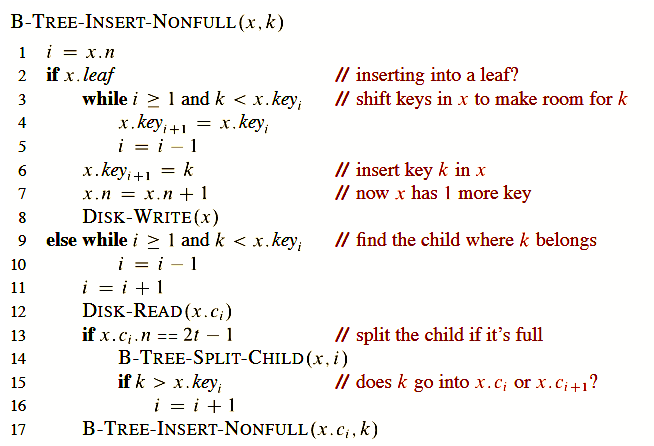
\includegraphics[width=.5\textwidth]{high-b-insert-no-full}
		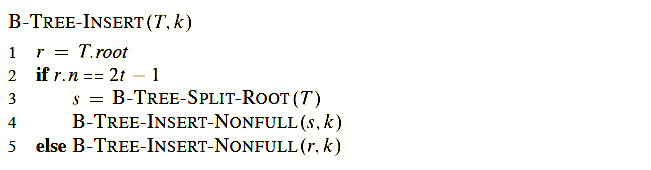
\includegraphics[width=.5\textwidth]{high-b-insert}
    \end{multicols}

    \begin{multicols}{2}
        \subsection{Rules}
        \begin{tabular}{r|cc|cc}\hline
            Node & Min & Max Deg & Min & Max Keys \\\hline
            Root & 0 & $2t$ & 1 & $2t-1$ \\ \hline
            Internal & $t$ & $2t$ & $t-1$ & $2t-1$ \\ \hline
            Leaf & \multicolumn{2}{c}{0} & $t-1$ & $2t-1$ \\ \hline
        \end{tabular}
        \subsection{Insertion}
        Start from root, split any full nodes. Then we can directly insert.
    \end{multicols}

    \subsection{Deletion}
    \begin{enumerate}
        \item[Case 1] At leaf --- delete
        \item[Case 2] Found in internal.
        \begin{enumerate}
            \item[Case 2a] Preceding child has $t$ keys: steal.
            \item[Case 2b] Succeeding child has $t$ keys: steal.
            \item[Case 2c] Adjacent children have $t - 1$ keys: merge into a $(2t - 1)$-key node, and recurse.
        \end{enumerate}
        \item[Case 3] Not found yet --- ensure next node has $t$ node for safe Deletion
        \begin{enumerate}
            \item[Case 3a] Preceding sibling has at least $t$ keys: steal.
            \item[Case 3b] Succeeding child has at least $t$ keys: steal.
            \item[Case 3c] Adjacent children have $t - 1$ keys: merge into a $(2t - 1)$-key node, and recurse.
        \end{enumerate}
    \end{enumerate}
    In case 2c and 3c, root can be empty after operation. We remove it.

    
    \section{Disjoint Set}
    \begin{tabular}{r|llll}\hline
        Method & Description & \textsc{Make-Set} & \textsc{Find} & \textsc{Union} \\\hline
        Array & Keep set ID             & ? & $O(1)$ & $O(n)$ \\ \hline
        Tree & Keep tree                & ? & $O(n)$ & $O(n)$ \\ \hline
        Linked-list & Keep head         & $O(1)$ & $O(1)$ & $O(n)$ \\ \hline
        Array &                         & ? & $O(1)$ & $O(n)$ worst case,  \\
        Small-to-Large &                &   &   &   $O(\log n)$ amortized \\ \hline
        Linked-list &                   & ? & $O(1)$ & $O(n)$ worst case, \\
        Small-to-Large &                &   &   & $O(\log n)$ amortized \\ \hline
        Tree Small-to-Large &           & ? & $O(\log n)$ & $O(\log n)$ \\ \hline
        Full &                          & $O(1)$ & $O(\log n)$ worst case, & $O(\log n)$ worst case,  \\
        &                               &   & $O(\alpha(n))$ amortized & $O(\alpha(n))$ amortized \\\hline
    \end{tabular}
    \clearpage

    \section{Hashing}
    \begin{itemize}
        \item \textbf{Direct-address tables}: Array ($h(x) = x$).
        \item \textbf{\textit{Uniform} hash function}: Probability of any probing sequence is the same (on slide).
        \item \textbf{\textit{Simple uniform} hash function}: $P(h(x) = a) = |U|^{-1}$
        \item \textbf{Load factor $\alpha$}: keys / slots
        \item \textbf{Division method}: $h(x) \equiv k \mod m$
        \item \textbf{Multiplication method}: $h(x) = \lfloor m (kA \mod 1) \rfloor = \lfloor m (kA - \lfloor kA \rfloor) \rfloor$
        \item \textbf{Quadratic probing}: $h(x, i) = (h'(x) + ai + bi^2) \mod m$
        \item \textbf{Double hashing}: $h(x, i) = (h_1(x) + i h_2(x)) \mod m$
        \item \textbf{Primary clustering}: Consecutive filled slots produced by open addressing probing
        \item \textbf{Secondary clustering}: IDK
        \item \textbf{Dynamic hashing using directories}: (left) When overflow occurs, duplicate table with unchanged pointers. Lazy resolve correct new hash until touched.
        \item \textbf{Directoryless Dynamic hashing}: (right) Lazy resolve collision, branch cell from 0 to full, and starts from 0 again (space doubled every scan), collision is solved only when the cell is duplicated.

        \begin{tikzpicture}[>=latex,scale=0.8,baseline={(2, 1.5)}]
            \draw[black] (0, 3) rectangle ++(1, 1) node[midway] {00};
            \draw[black] (0, 2) rectangle ++(1, 1) node[midway] {01};
            \draw[black] (0, 1) rectangle ++(1, 1) node[midway] {10};
            \draw[black] (0, 0) rectangle ++(1, 1) node[midway] {11};
            \draw[black] (1, 3) rectangle ++(2, 1) node[midway] {A};
            \draw[black] (1, 2) rectangle ++(2, 1) node[midway] {B, F};
            \draw[black] (1, 1) rectangle ++(2, 1) node[midway] {C, K};
            \draw[black] (1, 0) rectangle ++(2, 1) node[midway] {D};
        \end{tikzpicture}
        $\xrightarrow{\text{Insert G}}$     
        \begin{tikzpicture}[>=latex,scale=0.8,baseline={(2, 1.5)}]
            \draw[black] (0, 3) rectangle ++(1, 1) node[midway] {000};
            \draw[black] (0, 2) rectangle ++(1, 1) node[midway] {001};
            \draw[black] (0, 1) rectangle ++(1, 1) node[midway] {010};
            \draw[black] (0, 0) rectangle ++(1, 1) node[midway] {011};
            \draw[black] (0, -1) rectangle ++(1, 1) node[midway] {100};
            \draw[black] (0, -2) rectangle ++(1, 1) node[midway] {101};
            \draw[black] (0, -3) rectangle ++(1, 1) node[midway] {110};
            \draw[black] (0, -4) rectangle ++(1, 1) node[midway] {111};
            \draw[->] (1, 3.5) -> (2, 3.5);
            \draw[->] (1, 2.5) -> (2, 2.5);
            \draw[->] (1, 1.5) -> (2, 1.5);
            \draw[->] (1, 0.5) -> (2, 0.5);
            \draw[->] (1, -0.5) -> (2, 3.5);
            \draw[->] (1, -1.5) -> (2, 2.5);
            \draw[->] (1, -2.5) -> (2, -2.5);
            \draw[->] (1, -3.5) -> (2, 0.5);
            \draw[black] (2, 3) rectangle ++(2, 1) node[midway] {A};
            \draw[black] (2, 2) rectangle ++(2, 1) node[midway] {B, F};
            \draw[black] (2, 1) rectangle ++(2, 1) node[midway] {C, G};
            \draw[black] (2, 0) rectangle ++(2, 1) node[midway] {D};
            \draw[black] (2, -1) rectangle ++(2, 1) node[midway] {};
            \draw[black] (2, -2) rectangle ++(2, 1) node[midway] {};
            \draw[black] (2, -3) rectangle ++(2, 1) node[midway] {K};
            \draw[black] (2, -4) rectangle ++(2, 1) node[midway] {};
        \end{tikzpicture}
        \quad 
        \begin{tikzpicture}[>=latex,scale=0.8,baseline={(2, 1.5)}]
            \draw[black] (0, 3) rectangle ++(1, 1) node[midway] {00};
            \draw[black] (0, 2) rectangle ++(1, 1) node[midway] {01};
            \draw[black] (0, 1) rectangle ++(1, 1) node[midway] {10};
            \draw[black] (0, 0) rectangle ++(1, 1) node[midway] {11};
            \draw[black] (1, 3) rectangle ++(2, 1) node[midway] {A};
            \draw[black] (1, 2) rectangle ++(2, 1) node[midway] {B, F};
            \draw[black] (1, 1) rectangle ++(2, 1) node[midway] {C, K};
            \draw[black] (1, 0) rectangle ++(2, 1) node[midway] {D};
        \end{tikzpicture}
        $\xrightarrow{\text{Insert G}}$   
        \begin{tikzpicture}[>=latex,scale=0.8,baseline={(2, 1.5)}]
            \draw[black] (0, 3) rectangle ++(1, 1) node[midway] {000};
            \draw[black] (0, 2) rectangle ++(1, 1) node[midway] {01};
            \draw[black] (0, 1) rectangle ++(1, 1) node[midway] {10};
            \draw[black] (0, 0) rectangle ++(1, 1) node[midway] {11};
            \draw[black] (0, -1) rectangle ++(1, 1) node[midway] {100};
            \draw[black] (1, 3) rectangle ++(2, 1) node[midway] {A};
            \draw[black] (1, 2) rectangle ++(2, 1) node[midway] {B, F};
            \draw[black] (1, 1) rectangle ++(2, 1) node[midway] {C, K};
            \draw[->] (3, 1.5) -- (4, 1.5);
            \draw[black] (4, 1) rectangle ++(1, 1) node[midway] {G};
            \draw[black] (1, 0) rectangle ++(2, 1) node[midway] {D};
            \draw[black] (1, -1) rectangle ++(2, 1) node[midway] {};
        \end{tikzpicture} 
    \end{itemize}

    
\end{document}
